\section{Análisis de diferentes soluciones propuestas}
Vamos a proponer dos escenarios posibles para poder analizar sus soluciones. 

Estos dos escenarios los vamos a representar mediante un gráfico cada uno:
\begin{figure}[H]
    \centering
    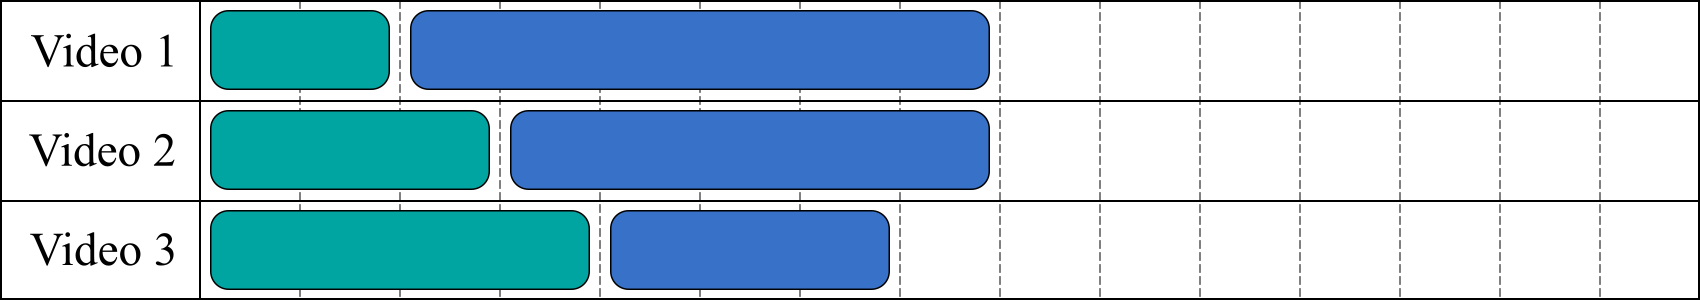
\includegraphics[width=1\textwidth]{img/caso-1-corto-largo.png}
    \caption{El tiempo que le tarda a Scaloni ver cada video es relativamente corto comparado con sus ayudantes.}
    \label{fig:Caso 1}
\end{figure}


\begin{figure}[H]
    \centering
    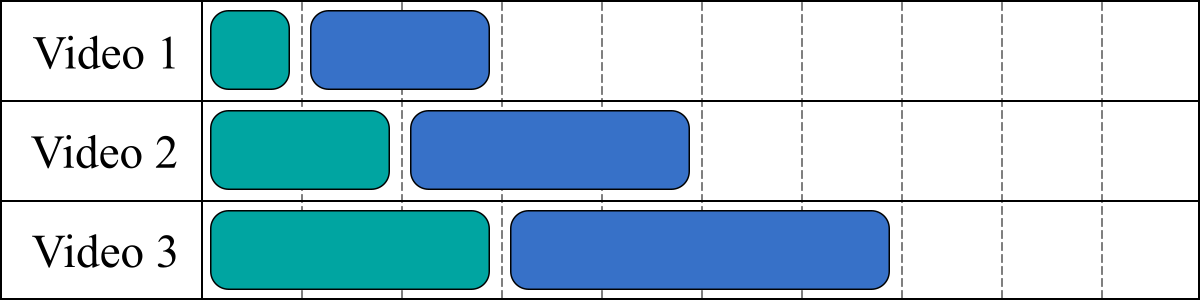
\includegraphics[width=1\textwidth]{img/caso-2-proporcionales.png}
    \caption{El tiempo que le tarda a los ayudantes ver cada video es proporcional a lo que le tarda a Scaloni.}
    \label{fig:Caso 2}
\end{figure}

En primer lugar, analizando ambos casos pudimos observar las siguientes características:
\begin{itemize}
    \item El orden en que Scaloni visualiza los compilados no incide 
    en el tiempo que le toma a él en finalizar la revisión de los mismos. 
    \item Minimamente, el tiempo final va a ser \sum_{k=1}^{n} s_k + a_n , siendo a_n el ayudante asignado a ver 
    el último video. Este caso es el más favorable de todos ya que supone que el ayudante que termina último en ver 
    el video es el último que empezó a verlo.
\end{itemize}

Tomando esto en cuenta, los algorítmos propuestos a continuación ignoran el tiempo que le tarda
al DT ver cada compilado. 

Para poder resolverlos se propusieron los siguientes algorítmos:

\subsection{Solución 1}

\begin{itemize}
    \item Ordenar los compilados de menor a mayor tiempo de análisis por parte de los ayudantes.
    \item Asignarle a Scaloni el compilado de menor tiempo de análisis por parte de los ayudantes, 
    y a medida que termina un compilado, que analice los demás en orden creciente.
    \item Asignarle a cada ayudante el compilado que acaba de terminar Scaloni.
\end{itemize}

\subsection{Solución 2 - La Solución Óptima}

\begin{itemize}
    \item Los asistentes realizan el análisis de cada uno de los compilados asignados en paralelo. Por lo 
tanto, el tiempo que se invierte en la revisión de un compilado específico de máxima duración, 
puede ser aprovechado de manera tal que este sea visto mientras Scaloni se dedica a la revisión
de otros compilados. De esta forma, nos aseguramos que se minimice el tiempo que suman los ayudantes 
en la resvisión total. 
    \item También en esta solución tiene en consideración el análisis 2 descripto previamente, ya que en el mejor de los casos,
    la \sum_{k=1}^{n} s_k + a_n termina siendo la mínima ya que, por la forma del ordenamiento del algorítmo, a_n es la duración del video más corto.

\end{itemize}

\textbf{Para ello propusimos el siguiente algoritmo:}

En primer lugar, hemos definido una clase llamada \texttt{Compilado} para modelar el compilado de cada 
oponente, con los atributos \texttt{tiempo\_scaloni} y \texttt{tiempo\_ayudante}, que almacenan 
el tiempo que le lleva analizarlo a Scaloni y a algún ayudante, respectivamente.

\begin{lstlisting}[language=Python]
class Compilado:
    def __init__(self, scaloni, ayudante):
        self.tiempo_scaloni = scaloni
        self.tiempo_ayudante = ayudante
\end{lstlisting}

De esta forma, y teniendo en cuenta los criterios previamente detallados, definimos la función
\texttt{compilados\_ordenados\_de\_forma\_optima} que recibe como parámetro un arreglo con
elementos de la clase \texttt{Compilado}. Esta ordena el arreglo en función del tiempo requerido
por los asistentes para visualizar cada compilado, en orden descendente. 

\begin{lstlisting}[language=Python]
def compilados_ordenados_de_forma_optima(compilados):
    return sorted(compilados, key=lambda compilado: compilado.tiempo_ayudante, reverse=True)
\end{lstlisting}

